\chapter{Integration of Transcriptomic and Proteomic data}
\label{sec:Integration}
The work presented in this chapter was done in collaboration with Dr James Wright,
Principal Bioinformatician within the Proteomics and Mass Spectrometry unit of the
Wellcome Trust Sanger Institute and Nuno Fonseca. James performed all the
identification and quantification of the proteins, which also includes the
implementation of the new method of protein quantification presented in the
Section~\ref{sec:IntegrationNewMethQuant}. Nuno performed the quality
control, the mapping and the quantification of the \dataset{Gtex} data.
I have performed the quality control, the mapping and the quantification of the
\dataset{Uhlén \etal} dataset. I have also performed
all the data analysis and integration under the supervision of Dr Alvis Brazma
(EMBL-EBI) and Dr Jyoti Choudhary (Wellcome Trust Sanger Institute).

A manuscript describing this work is being prepared with the other authors.

\section{Introduction}
\label{sec:IntegrationIntro}
%%--- \textit{or why we bother with integration?}}
%
%    here should be explain all the reasons and the challenging of why this is
%    important.
%    Here some of the reasons: transcriptomics and proteomics are not the same
%    range (technology bias)
%    It is hard to say when it is NOT correlated if this comes from a
%    technical problem or regulation.
%
%    Workflows a lot better established in transcriptomics than proteomics
%    (annotation, mapping)
%%%%%

The core of central dogma of molecular biology --- i.e.\ one \DNA\ (coding) gene
will be transcribed as one \mRNA\ transcript and will be in turn translated in
one protein --- still holds true even though we now know the truth is not as
linear as we thought first. Many regulation processes are implied before
and after the transcription and translation steps.
In the figure~\ref{dogma} which is the reconstruction by~\cite{Crick:1958} of
what was conceived circa 1958: the solid lines present the proven mode of
information transfers, the dashed ones are the ones that were postulated but
have yet to be proven. To update this figure to our current knowledge, the line
starting from the RNA to the DNA should be a solid one.

\begin{figure}[!htbp]
    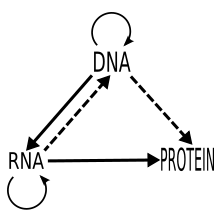
\includegraphics[scale=0.6]{integration/dogma}\centering
    \caption{\label{dogma}Central dogma of molecular biology proposed by F. Crick
    circa 1958}
\end{figure}

However, as we still have to prove that proteins can be produced directly
from \DNA\footnote{which seems pretty unlikely to me}, it is assumed that
each protein is created by translation, hence studying
transcriptomics and proteomics together for the same conditions should give us
insights on these regulation processes.

Whereas it was implicitly assumed for a long time that for similar conditions
there should be a proportional relationship between transcriptomics and
proteomics, many studies\
\fixme{add references, see TAC report 3}
done in cells have failed to show high correlation between the two biological
layers. From then, while there are still studies done jointly on transcriptomics
and proteomics, the focus has greatly shift either on the presence or absence of
a protein/transcript in a specific condition or if both transcript and protein
are differential expressed between two conditions in the same way.
Nowadays, there are not many efforts to directly link their actual expression.

Previous studies did not managed to show correlation between proteomics and
transcriptomics above 0.5 (Pearson correlation coefficient).
However, while cell populations could have external factors impacting their
overall expression, an easy assumption is that tissue samples should be driven
by their function first. As such we expect that what makes a liver a liver and
what makes a heart a heart would overcome most of the technical variability.

In fact, here, even though I have only access to independent data, the average
Pearson correlation per tissue is above 0.5
[min: 0.45 (Oesophagus); max: 0.666 (Liver)].

In 2014, two large proteomics assays focusing on normal human tissues have been
released for the first time.
\fixme{add citation for Pandey and Kuster}
Until now, there was not such availability of large-scale and extensive tissues
both on transcriptomic and proteomic layer to jointly study the genes
translation into proteins across a consequent set of tissues
at the same time. Alike the \dataset{Uhlén \etal} dataset and the \dataset{Gtex}
these datasets have not the same scope of tissues. However, the overlap of
studied tissues is enough to draw an overview of the current technology.


In their review,~\cite{Uhlen:2016}, the authors outline one on-going debate
in the literature, which could be formulated whereas we should observe (or not)
good correlations between proteomic and transcriptomic data.
Indeed, first investigations found low or no correlation. More recent
studies reported improved correlations although these correlations were around
0.4 (Pearson correlation coefficient). Such discrepancies could be explained
partially by the difference of the technology for proteomic and transcriptomic
assays. Sequencing-based technologies, as \Rnaseq\, enhanced greatly the
assessment of transcripts. While true absolute quantification is not reached yet, there is not saturation any more or, more importantly, out-of-scope issues as
they could have been observed with microarrays. In theory, on one hand, with
enough sequencing depth, every transcript expressed in a cell or tissue could be
catch by high-throughput sequencing and in the other hand, two transcripts with
different level of expression would be differentiate whereas they are very highly
expressed or not. If there is a difference in their level of expression, this
difference should be catch.

Unfortunately, technology on the proteomic side is not as advanced yet.
Mass spectrometry is still one of the most accurate ways to quantify the
abundance of proteins. However, often the top 25 most abundant proteins can
amount for more than 50\% of the signal collected for a sample. Therefore, the
identification (and hence quantification) of the scarcer proteins is harder.
\fixme{find reference -> ask Jyoti}

\fixme{see bottom of page2 in the paper}

These technical divergences and specificities call for an underlying premise:
when is a specific protein or transcript considered as expressed in a dataset?
In a particular tissue? This premise is discussed
in the Section~\ref{sec:IntegrationExpressedOrNot}.



\section{Data}
\label{sec:IntegrationData}
While the \dataset{Kuster} dataset presents more tissues in common
with the Gtex and Uhlén datasets (see figures~\ref{VennTissuePandeyGtexUhlen}
and~\ref{VennTissueKusterGtexUhlen}), I had focused the study on
the \dataset{Pandey \etal} dataset. Indeed, we managed to quantify the biggest number
of proteins in this later dataset: 10272 proteins across 24 samples for
\dataset{Pandey} versus 7223 across 24 samples for \dataset{Kuster}\footnote{Even
if the number of samples is the same for the \dataset{Pandey} and
the \dataset{Kuster} datasets, this is purely fortuitous.}.
This has an increased importance as the study goes beyond the correlation of
proteomics and transcriptomics for a same tissue. The number of proteins
detected within a tissue is also greater for \dataset{Pandey} as shown
in figure~\ref{KusterPandeyFQM} (A and B).
It worth noticing that even there is the same number of samples for the
\dataset{Pandey} and the \dataset{Kuster}, this is purely fortuitous.

Furthermore, all the \dataset{Pandey} data has been
collected on the same platform while the \dataset{Kuster} data has been
collected on different ones. On a side note, as each of the proteomic datasets
proposes only one sample per tissue, it is difficult to assess if the good or bad
correlation between the Kuster \etal\ or the Pandey \etal\ proteomic data
and the available transcriptomic data is due to the technology or
to the nature of the tissue.

Besides, as the datasets \dataset{Pandey} and \dataset{Uhlén} presents 15 common
tissues, which includes 12 common tissues with \dataset{Gtex}, if not
indicate otherwise, the following results are based on the first combination of
datasets. As the whole analysis pipeline as been applied to the three datasets
for the same 12 tissues, some of the figures have a counterpart in the
appendices displaying the results for all three datasets when focusing only on
that smaller subset of tissues. To ease the comparison, the references of the
supplementary figures are given in green (and in brackets) in the legend of the
main one. Overall, the main results and conclusions remain the same either if
I use Gtex or Uhlén \etal\ data.




\begin{figure}[!htbp]
    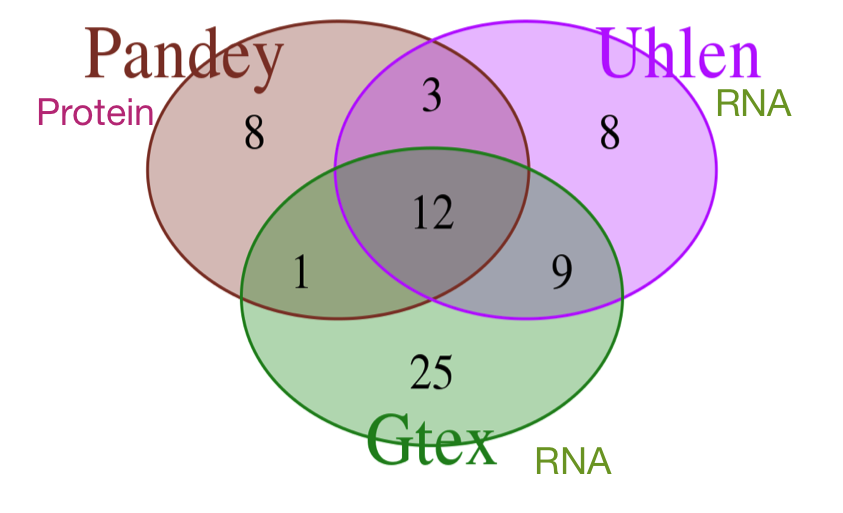
\includegraphics[scale=0.65]{integration/PandeyGtexUhlen_tissuesVenn.png}
    \centering
    \caption{\label{VennTissuePandeyGtexUhlen}Number of share and unique
    tissues between the proteomic dataset
    from Pandey \etal\ and the transcriptomic datasets (Uhlén \etal\ and Gtex)}
\end{figure}

\begin{figure}[!htbp]
    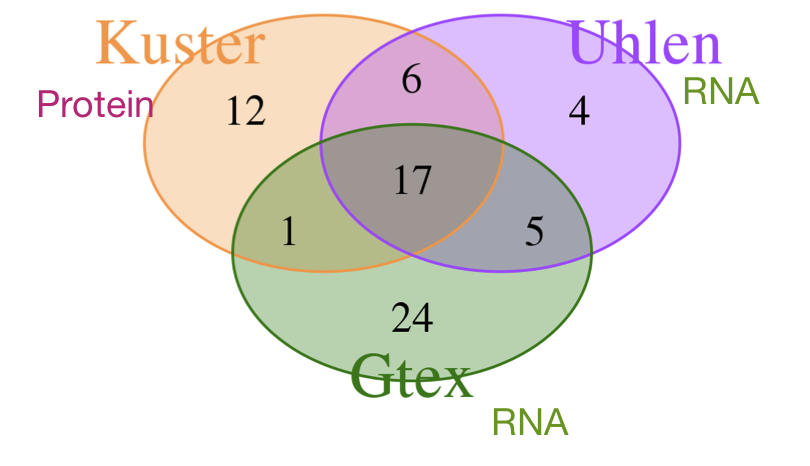
\includegraphics[scale=0.65]{integration/KusterGtexUhlen_tissuesVenn.png}
    \centering
    \caption{\label{VennTissueKusterGtexUhlen}Number of share and unique
    tissues between the proteomic dataset
    from Kuster \etal\ and the transcriptomic datasets (Uhlén \etal\ and Gtex)}
\end{figure}


\begin{figure}[!htbp]
    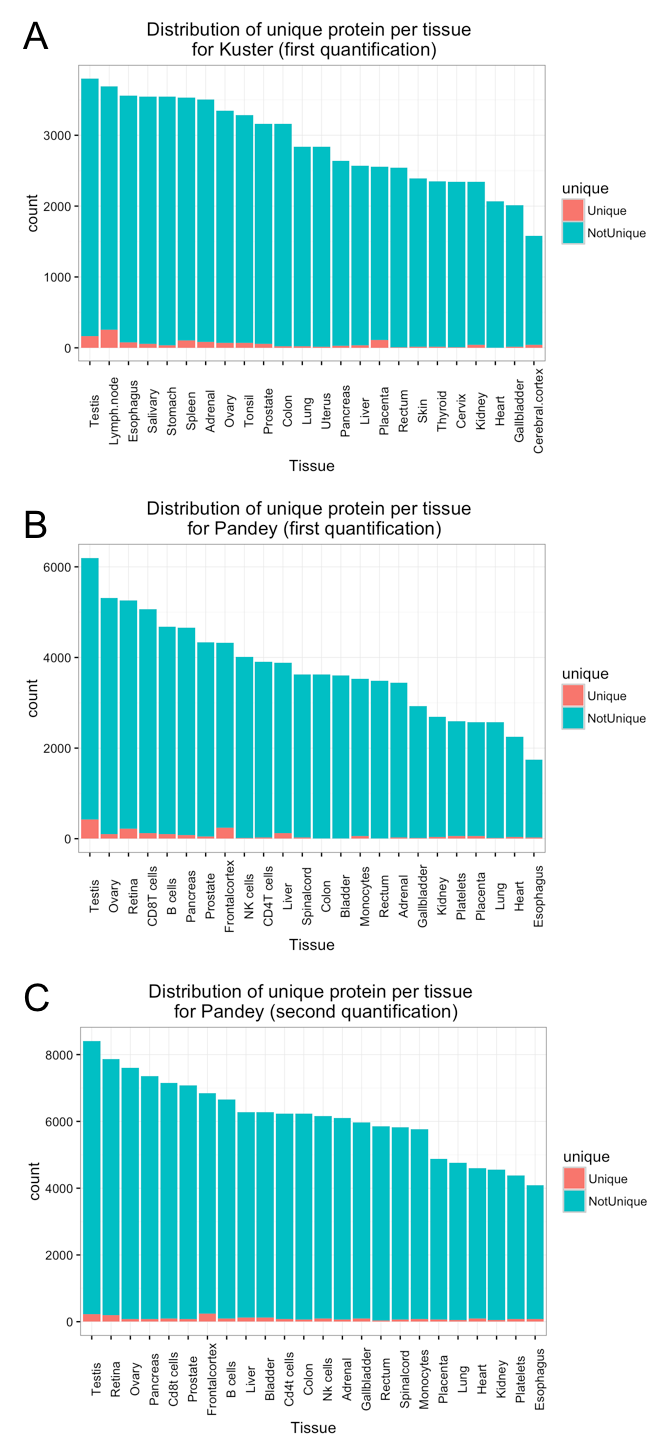
\includegraphics[scale=0.92]{integration/KusterPandey1_2FQM.png}\centering
    \caption{\label{KusterPandeyFQM}Distribution of proteins across the tissues.
    Highlighted in red are the proteins that are found only in that
    tissue within the dataset. A| Kuster (first quantification method).
    B| Pandey (first quantification method).
    C| Pandey (second quantification method).}
\end{figure}


\section{Expressed or not expressed}
\label{sec:IntegrationExpressedOrNot}

While it can seem as a trivial concept and might be overlook, whether a specific
molecule is expressed --- or not --- in a given condition, can actually have
an extensive impact on the results of the integration.

Indeed, the Pearson correlation is very sensitive to outliers and null values,
\fixme{Add reference}
hence it is important that all the data used for the analysis is meaningful.

\subsection{The undefined}
\label{sec:IntegrationExpressedOrNot-undefined}
If a protein or transcript is never found in any of the samples of a dataset,
then I considered that we can not determine if the protein or transcript was
either truly not expressed or, for any reason, was not capture while the library
preparation or the identification/quantification steps. Hence, those are
excluded from the analyses as I can not resolve precisely if this is a
technical artefact or a biological truth.

\subsection{Expression in a dataset}
\label{sec:IntegrationExpressedOrNot--expDataset}
By contrast, if a protein or a transcript is expressed in any sample of the
dataset, then, whenever there wasn't any expression recorded in the other
samples, I consider that the expression of the considered macromolecule is truly
null for those samples.

\subsection{Expression within a sample}
Due to the technical (and biological) differences between proteomics and
transcriptomics, I use different thresholds to define the expression of a protein
or a transcript.


\subsubsection{Expressed protein}
On the proteomic side, I consider that a protein is expressed if it has been
identified and quantified. In other words, if the expression value of a protein
is greater than zero in a sample, I consider it as expressed.

\subsubsection{Expressed transcript}
It is a bit more complex on the transcriptomic side as there can be
\fixme{find reference on translational noise in RNAseq}
translational noise. While this noise could be evaluate by empirical methods for
each \Rnaseq\ dataset, there is a widespread threshold used in the literature:
1 \gls{FPKM}/\gls{RPKM}. In fact,~\cite{Hebenstreit:2011} showed in
their study \paper{RNA sequencing reveals two major classes of gene expression
levels in metazoan cells}, that to be translated into a protein, a \mRNA\ should
present an expression at least equals to 1 \gls{RPKM}.

As our current study focuses on the comparison of proteomic and transcriptomic
data, all the analyses have been run with this threshold. It is worth mentioning
that parts of the analyses have also been done either without
any threshold (i.e.\ the same definition used with the proteins has been applied)
or with a threshol of 5 \gls{FPKM}.

\subsection{Limitation of the current study}

There are two main constraints, I would like to highlight.

First, as there is only one sample per tissue in the \dataset{Pandey \etal}
dataset, the expression found in one sample is \textit{de facto} the proteomic
expression. On the other hand, the \dataset{Uhlén \etal} have \emph{technical}
and \emph{biological} replicates for each tissue. To calculate the expression
used for each tissue, I used the median\footnote{When there were more than
two samples, otherwise it is the mean of expression of the two biological
replicates} of the transcript expression after having computed the mean of its
expression for the technical replicates of each individual.


Secondly, while I have compared the list of \emph{undefined} transcripts and
proteins (between \dataset{Pandey \etal} and \dataset{Uhlén \etal} data and
between \dataset{Pandey \etal} and \dataset{Gtex}), I have done the bulk of the
analyses on pairwise (or three-way) \emph{defined} protein and \mRNA(s).

In other words, if the proteins and their corresponding transcripts are not
expressed at least in one sample in each dataset, they are unfortunately excluded
from many many steps of the analysis workflow.

\section{Results}
\label{sec:IntegrationResults}

For this study, the processed \dataset{Uhlén \etal} and \dataset{Gtex} datasets
used are a subset of the processed data previously presented in the
Chapter~\ref{sec:Transcriptomics} (see: Section~\ref{sec:Trans_ReproExpresTissue}
for the processing methods). Indeed, only the common set of tissues with the
\dataset{Pandey \etal} study and the genes with a biotype annotated as protein
coding in the Ensembl 76 released are kept.

I ran the analyses on both quantification (HTSeq and Cufflinks); if not stated
otherwise the quantification used for the figures are based on the normalised
\glspl{FPKM} output of HTseq.


In the same fashion as the transcriptomic data that have been reprocessed before
being employed in our studies, the proteomic data have been reprocessed
by James from the raw files he has downloaded from ProteomeXchange
(\cite{ProteomeXchange:2014}) via the PRIDE database (\cite{Pride:2016}).
\fixme{Ask James for the methods}

The common tissues between \dataset{Pandey \etal} and \dataset{Gtex} are
(by alphabetical order):  Adrenal gland, Bladder, Colon, Oesophagus, Heart,
Kidney, Liver, Lung, Ovary, Pancreas, Placenta, Prostate and Testis.

The common tissue between \dataset{Pandey \etal} and \dataset{Uhlén \etal} are
an enlarged version of the previous set, with the addition of Gall bladder,
Placenta and Rectum.

\subsection{New quantification method for the proteomic data}
\label{subsec:IntegrationNewMethQuant}

\textit{Quantifications performed by Dr James Wright}

At first, the quantification used for the proteomic data was following
state-of-the-art protocols for which we applied very stringent parameters:
to identify and quantify a given protein, three different unique peptides
(with a \gls{FDR} < 0.01 \%) have to be mapped solely to that protein. A main
issue of this approach is that many proteins have similar sequences; hence, some
peptides can only be attributed to clusters of proteins. A naive approach would
be to aggregate the corresponding transcriptomic expressions together to enable
the comparison\footnote{Which then would also require further steps of
normalisation on the transcriptomic part.}. However, we found that the cluster
of peptides/proteins are not consistent from one study to another. Indeed, we do
not always observe the same set of peptides and, moreover, the proteins clusters
they support are quite different. That is why I have not investigate this option
further as for each study I would need a new aggregate annotation as a reference.
It would be then be quite difficult to assess the discrepancy due to the
variations of aggregation. For this method of quantification, I choose to exclude
the cluster of peptides/proteins from the study. Since I also work with a subset
of the tissues, the number of quantified proteins could seem a bit low compare
to the original study.

After discussions where we were comparing the different quantification algorithms
and methods used for \Rnaseq\ data, we have decided to try a new quantification
method\footnote{Inspired by algorithms as Cufflinks} for the proteomics:
the amount of proteins would still take in account the \emph{unique} peptides,
but also the peptides that could be attributed to several proteins.
These \emph{ambiguous} peptides are then probabilistically assigned to the
mapped proteins they are more likely to come from (based on the distribution of
the other peptides that could be mapped to each protein).

Both quantification methods have been implemented by James Wright.

In the context of this work (i.e.\ when focusing on the 15 common tissues between
the \dataset{Uhlén \etal} and the \dataset{Pandey \etal} datasets),
he has quantified about 6,400 proteins with
the standard method. With the new method, he has quantified a bigger set of
proteins: about 12,300 proteins.

As shown in figure~\ref{KusterPandeyFQM} (B and C),
all tissues and cell lines benefits from this new quantification and there isn't
any tissue or cell line that is dramatically impacted compared to the others.

I have performed the analyses presented in this chapter on both sets of
quantification. As the high-level results and conclusions are remaining the same,
the figures and discussions hereafter are based on
the new quantification method. For comparison purposes,
I have produced (following the same analyses and their associated implementations)
some figures and tables from the data quantified by the first method.
Those can be found in the appendices; their references
are given in blue (and in brackets) in the caption of the main figures.


\textbf{N.B.:} Considering that the scale of expression between
the proteomic assay and the transcriptomic ones is not directly comparable,
all the data (regardless of the method of quantification) have been transformed
with $X_{i}=\log_{2} (x_{i}+1)$ before any other computation or visualisation.

\subsection{Expression profile of proteomics and transcriptomics look very
similar in shape}
\label{sec:IntegrationExpProfileSim}

As discussed in the previous chapters, visualising the data is very important
prior to any computation. It allows to detect if we are violating
any assumption or if there is any issue with the data. In fact, we have seen in
Chapter~\ref{sec:Transcriptomics} that there is an issue with the pancreatic
samples, as the range of genes expression is quite different from the other
samples/tissues.

In the following sections, we consider the new quantification method for the
proteomic data and compare it to the \dataset{Uhlén \etal} dataset for the
15 common tissues.

As shown in figure~\ref{VennGeneTransProt15}, there are 14,617 pairs of
proteins/genes. While, we expect a greater number of transcripts than proteins,
it could however be primarily surprising that there are proteins
(See~\ref{sec:protNoTransTable}) which don't have
a match in the transcriptomic data. There are actual several possible explanations.

It could be a technical issue or an artefact on the transcriptomic side, e.g.\:
the \mRNAs\ were present but were not capture for a reason or another at the
library preparation; the \mRNAs\ have a high sequence-similarity with other \mRNAs\
and the reads haven't been accurately assigned; the lacking \mRNAs\ are not properly
annotated in the version of the genome I used at the mapping step.

It might also be that the protein doesn't belong to the sample: the identification
is a false positive or incorrect; the sample\footnote{Or the instrument used for
the capture} could also been contaminated at some point with some foreign proteins.

It can also be due to an underlying biological phenomenon:
the turnover of the \mRNA\ is very low and the protein is very stable; the proteins
have been expressed somewhere else in

\begin{figure}
    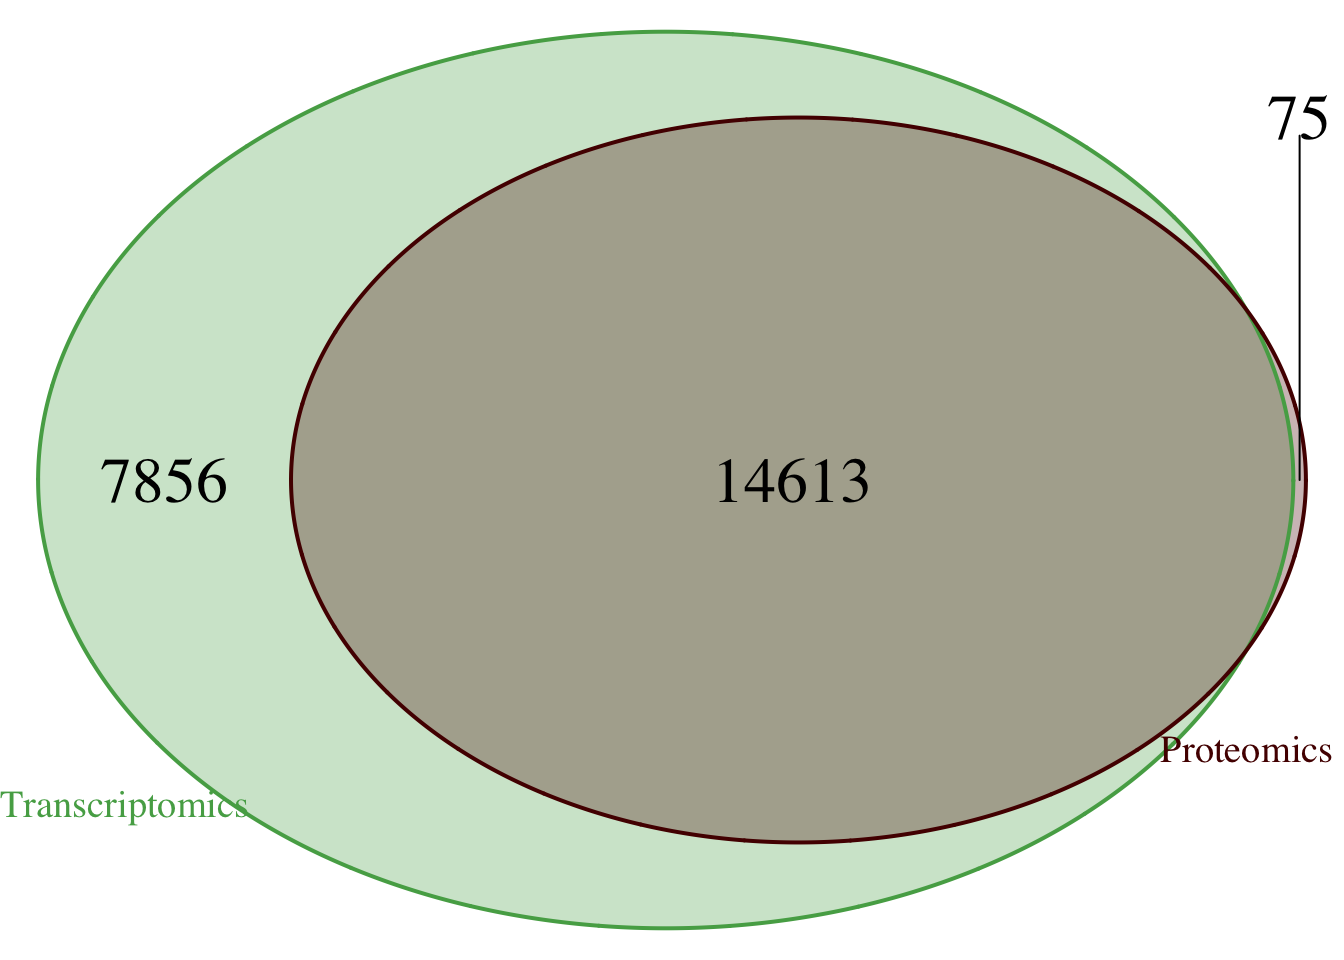
\includegraphics[scale=0.15]{integration/VennGeneTransProt15}\centering
\caption{\label{VennGeneTransProt15}Unique and shared protein/gene pairs between
    Proteomics and Transcriptomics (Pandey \etal\ (PPKM) and Uhlén \etal\
    (\gls{FPKM}) data)} \subcap{There are 14,613 pairs common between the
    transcriptomic and the proteomic dataset.}
\end{figure}


\begin{figure}%[!htbp]
    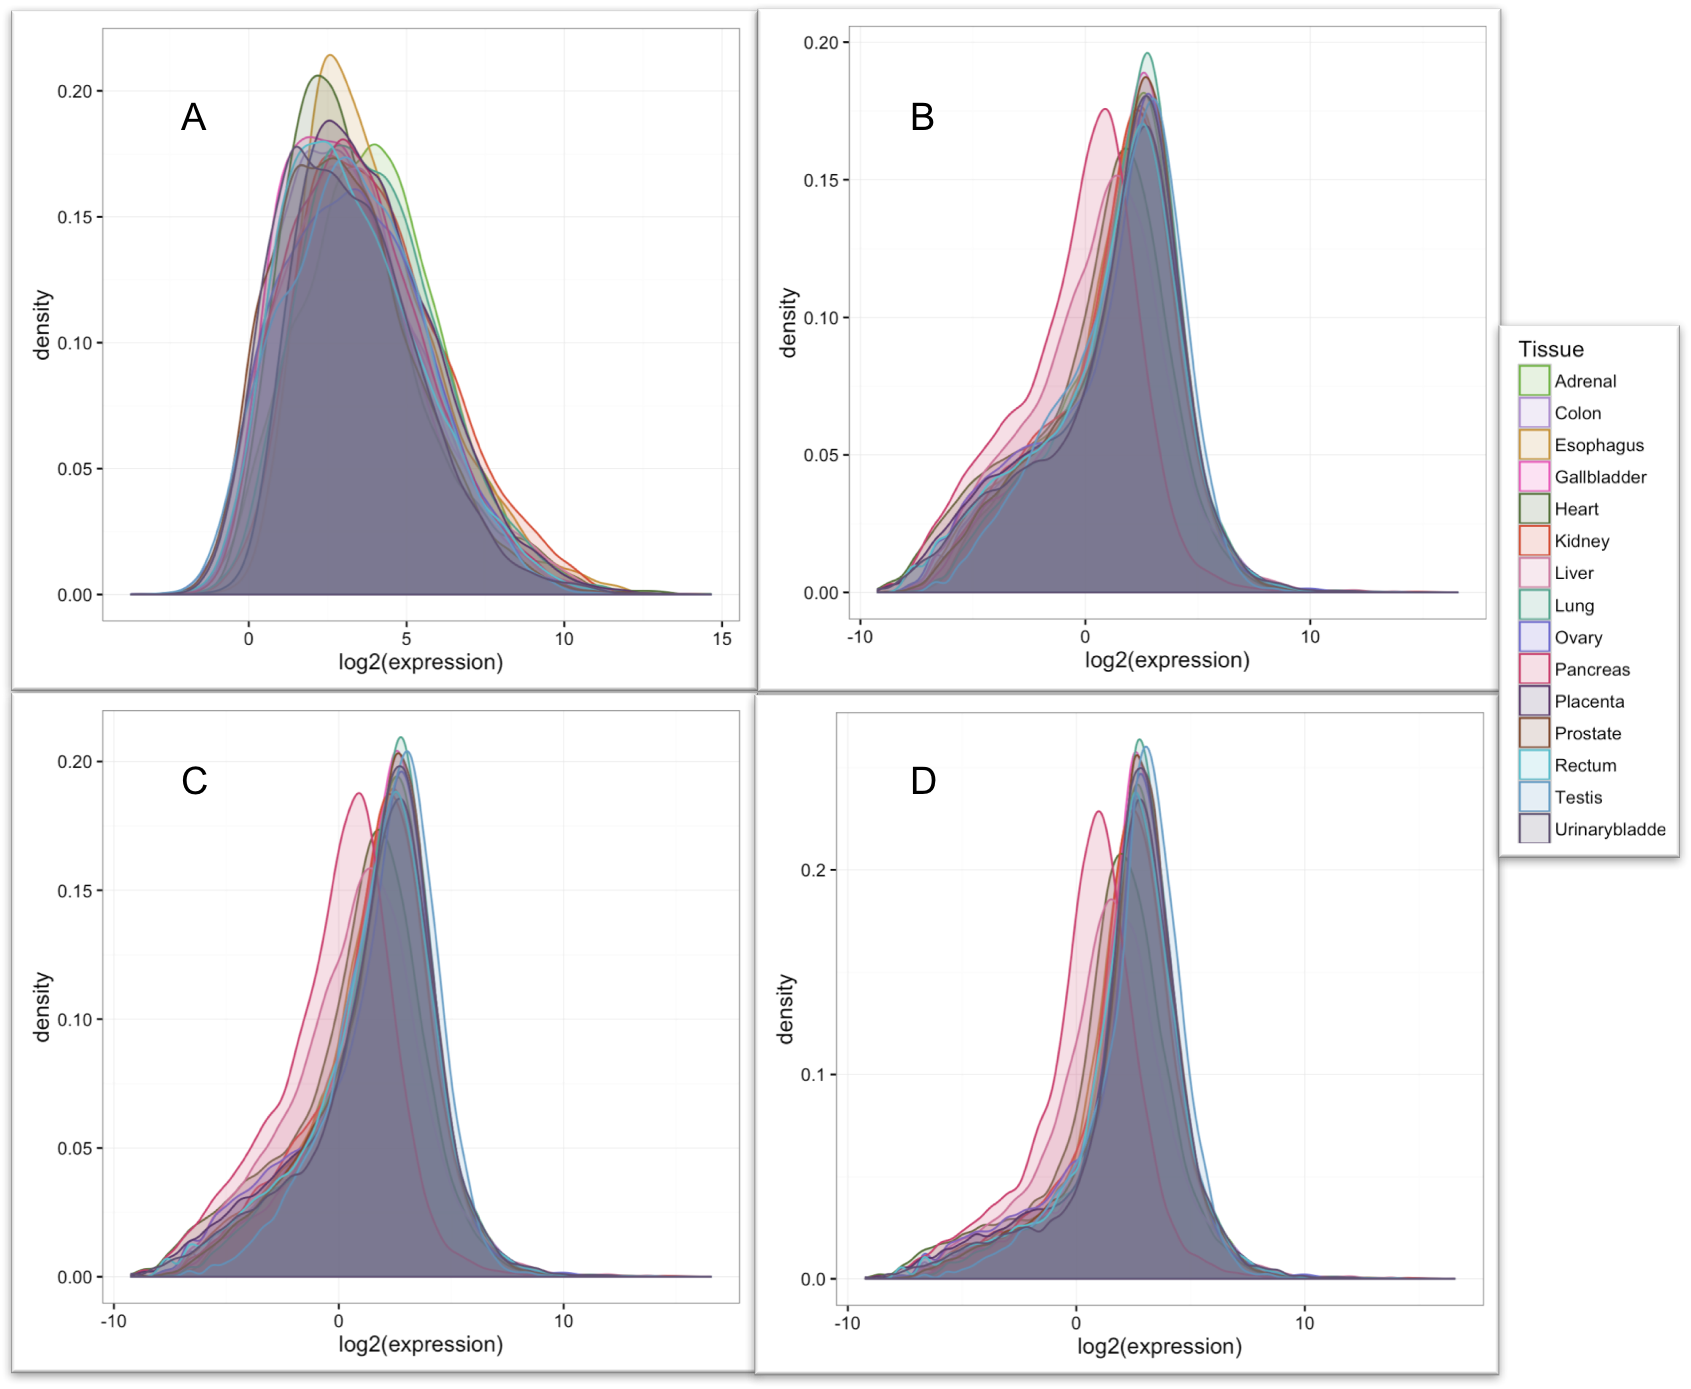
\includegraphics[scale=0.45]{integration/densityExpProtTrans15}\centering
    \caption{\label{densityExpProtTrans15}Density of expression of proteins
    (\textbf{A}) and \mRNAs\ (\textbf{B},\textbf{C},\textbf{D}) per tissues.}
    \subcap{\textbf{B},\textbf{C},\textbf{D} presents the same data but with
    different thresholds; respectively: No threshold, 1 \gls{FPKM} and
    5 \glspl{FPKM}. The threshold used for the proteins is the threshold of
    detection (i.e.\ greater than 0). The different density of distributions are
    globally gaussian. When the threshold is increased for the transcriptome, the
    shape get closer to the ideal one, as the bulge created by lowly expressed
    genes is removed. We can also observe that the problem with the pancreatic
    tissue get more highlighted with higher thresholds.}
\end{figure}


 \begin{figure}%[!htbp]
     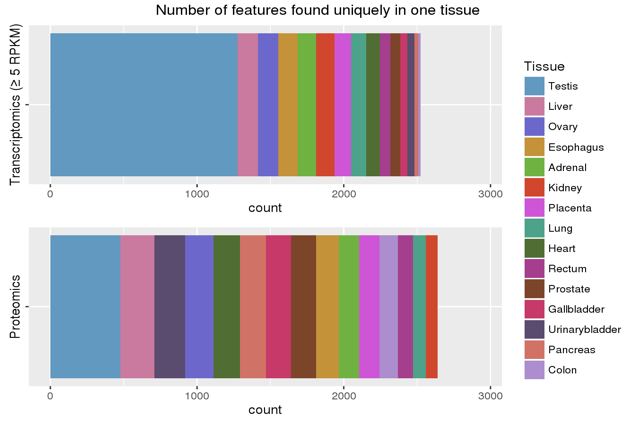
\includegraphics{integration/barPlotunique}\centering
     \caption{\label{barPlotunique} Number of \mRNAs\ (top) and proteins (bottom)
     that have been detected and quantified (\geq\ 5 \glspl{FPKM} for \mRNA\; > 0
     for proteins).} \subcap{While some tissue can have consistently a higher
     specificity at proteomic and transcriptomic level, it is not true for all.}
 \end{figure}







\subsubsection{Comparable density of expression profiles per tissue}
Figure~\ref{densityExpProtTrans15} presents the density of expression
of proteins and \mRNAs\ per tissue. In~\ref{densityExpProtTrans15}|A,
we notice that 


\subsubsection{Distribution of expression breadth of the proteome is bimodal. As is
the expression breadth of the \mRNAs\ --- if we apply a threshold}

Most proteins are detected in a small number of tissues or in all the tissues.
For the transcriptome, if we focus only on the detected genes, we don’t see
such trend. However, when we apply a threshold (1 \gls{FPKM} or 5 \glspl{FPKM})
above which the \mRNAs\ have to be expressed to be counted, then their distribution
of expression breadth is also bimodal.

We can also note that while for some tissues having a bigger diversity of
specific proteins mean to have a broader diversity at transcriptomic level,
it is not true for all the tissues as displayed in
figure~\ref{integration/barPlotunique}.


\label{sec:IntegrationProteinBimodalExpre}
\fixme{this might need to go to the previous chapter!}




\subsection{Independent transcriptomic and proteomic studies of normal
human tissues have good and significant correlation}
\label{sec:IntegrationGoodCorrProtTrans}


\fixme{add figure 10 and 11 from 3rd TAC?}



 ranking the expression
Tissue correlation
Tissue specific genes/proteins – how consistent they are in RNA and proteomics?
Gene correlation
Correlated and uncorrelated genes, what is specific to each group
functional groups of genes


\subsection{Consistency of expression at tissue level}
\subsection{Consistency of expression at gene level}
\subsection{Specificity,House-keeping genes}
\subsection{Genes functionality impact}
\subsection{Annotation impact}



\section{Discussion}
\section{Conclusion}


%%%%cimetiere
%%These studies however were mostly done at cell levels.
%%While the pool of protein coding transcripts is about 60 to 70 \% similar from
%%one tissue to another, the protein pool is quite different.




